% WCom Theory project report.
% Upload this whole folder (main.tex, numbers.tex, ris_sim.py, figures/) to Overleaf
% and compile with pdfLaTeX.
\documentclass[11pt,a4paper]{article}
\usepackage[margin=1in]{geometry}
\usepackage[T1]{fontenc}
\usepackage[utf8]{inputenc}
\usepackage{lmodern}
\usepackage{amsmath,amssymb,bm}
\usepackage{graphicx}
\usepackage{booktabs}
\usepackage{float}
\usepackage{caption}
\usepackage{enumitem}
\usepackage{xcolor}
\usepackage{listings}
\usepackage[hidelinks]{hyperref}

\graphicspath{{figures/}}
\setlength{\parskip}{0.5em}
\setlength{\parindent}{0pt}
\captionsetup{font=small,labelfont=bf}

\lstset{language=Python,basicstyle=\ttfamily\scriptsize,breaklines=true,
  keywordstyle=\color{blue!60!black},commentstyle=\color{green!40!black},
  stringstyle=\color{red!60!black},numbers=left,numberstyle=\tiny\color{gray},
  frame=single,framerule=0.3pt,columns=fullflexible}

% Shorthand
\newcommand{\hrv}{\bm{h}_r}
\newcommand{\hdv}{\bm{h}_d}
\newcommand{\Gm}{\bm{G}}
\newcommand{\wv}{\bm{w}}
\newcommand{\vvec}{\bm{v}}
\newcommand{\Thm}{\bm{\Theta}}
\newcommand{\Phm}{\bm{\Phi}}
\newcommand{\Rm}{\bm{R}}
\newcommand{\Vm}{\bm{V}}
\newcommand{\udBm}{\,\text{dBm}}
\newcommand{\udB}{\,\text{dB}}

% All numbers quoted from our simulations live in numbers.tex, which is
% written by simulation/make_numbers.py from figures/results.json.
% Generated by simulation/make_numbers.py from figures/results.json. Do not edit by hand.
\newcommand{\Msim}{4}
\newcommand{\Nsim}{40}
\newcommand{\nReal}{1000}
\newcommand{\nSdr}{200}
\newcommand{\nRand}{1000}
\newcommand{\peakD}{40}
\newcommand{\peakP}{8.3}
\newcommand{\aoFifty}{\ensuremath{-3.6}}
\newcommand{\noIrsFifty}{14.8}
\newcommand{\saveFifty}{18.4}
\newcommand{\gapLB}{less than 0.01}
\newcommand{\gapUserMRT}{7.3}
\newcommand{\gapIrsMRT}{12.5}
\newcommand{\gapRand}{15.6}
\newcommand{\dropA}{5.7}
\newcommand{\dropB}{5.9}
\newcommand{\dropFifteen}{0.4}
\newcommand{\gapRay}{less than 0.01}
\newcommand{\lossOne}{3.8}
\newcommand{\lossTwo}{0.9}
\newcommand{\aoNtwenty}{1.9}
\newcommand{\aoNthirty}{\ensuremath{-1.3}}
\newcommand{\aoNsixty}{\ensuremath{-6.9}}
\newcommand{\paperNoIrs}{19.19}
\newcommand{\paperNtwenty}{4.49}
\newcommand{\paperNthirty}{1.49}
\newcommand{\paperNsixty}{\ensuremath{-4.06}}
\newcommand{\offNoIrs}{4.4}
\newcommand{\offNtwenty}{2.6}
\newcommand{\offNthirty}{2.8}
\newcommand{\offNsixty}{2.9}
\newcommand{\dropPaper}{5.6}
\newcommand{\dropPaperFig}{5.5}
\newcommand{\closedNoIrs}{14.7}
\newcommand{\plNoIrs}{19.48}
\newcommand{\offPl}{\ensuremath{-0.29}}
\newcommand{\gainLoS}{6.7}
\newcommand{\gainRay}{4.9}
\newcommand{\ciExpOne}{1.6}
\newcommand{\ciExpOneRest}{0.7}
\newcommand{\ciExpTwo}{0.25}
\newcommand{\lossThree}{0.2}
\newcommand{\tableDist}{%
\begin{tabular}{lrrrrrr}
\toprule
Scheme & $d=15$\,m & $d=25$\,m & $d=35$\,m & $d=43$\,m & $d=47$\,m & $d=50$\,m \\
\midrule
Lower bound (SDR) & $\ensuremath{-3.3}$ & $3.7$ & $7.9$ & $7.7$ & $3.5$ & $\ensuremath{-3.6}$ \\
SDR + randomisation & $\ensuremath{-3.3}$ & $3.7$ & $7.9$ & $7.7$ & $3.5$ & $\ensuremath{-3.6}$ \\
Alternating optimisation & $\ensuremath{-3.3}$ & $3.7$ & $7.9$ & $7.7$ & $3.5$ & $\ensuremath{-3.6}$ \\
AP--user MRT & $\ensuremath{-3.3}$ & $3.7$ & $8.2$ & $9.3$ & $7.6$ & $3.8$ \\
AP--IRS MRT & $9.2$ & $12.1$ & $12.9$ & $9.4$ & $3.9$ & $\ensuremath{-3.5}$ \\
Random phase shift & $\ensuremath{-3.2}$ & $4.1$ & $9.2$ & $12.4$ & $13.4$ & $12.0$ \\
Without IRS & $\ensuremath{-3.2}$ & $4.1$ & $9.2$ & $12.5$ & $14.1$ & $14.8$ \\
\bottomrule
\end{tabular}}
\newcommand{\tableEnv}{%
\begin{tabular}{ll}
\toprule
Item & Version / setting \\
\midrule
Python & 3.12.13 \\
NumPy & 2.4.3 \\
CVXPY & 1.9.3 \\
SCS (SDP solver) & 3.3.2 \\
Matplotlib & 3.10.8 \\
Solver settings & SCS via CVXPY, eps = 1e-5, default other settings \\
Operating system & macOS 27.2.1 (arm64) \\
Processor & Apple M2, 8 cores \\
Random seed & 2026 \\
\bottomrule
\end{tabular}}


\begin{document}

%-----------------------------------------------------------------------------
\begin{titlepage}
\centering
{\large The LNM Institute of Information Technology, Jaipur\par}
{\large Department of Communication and Computer Engineering\par}
\vspace{2.5cm}
{\Large Wireless Communication (Theory) \\[2pt] Project Report\par}
\vspace{1.5cm}
\rule{\linewidth}{0.6pt}\\[10pt]
{\LARGE\bfseries Intelligent Reflecting Surface Enhanced Wireless Network via Joint Active and Passive Beamforming\par}
\vspace{6pt}
{\large A study and simulation-based reproduction\par}
\rule{\linewidth}{0.6pt}
\vspace{1.2cm}

{\large Paper studied\par}
\vspace{4pt}
Q.~Wu and R.~Zhang, \emph{IEEE Transactions on Wireless Communications},\\
vol.~18, no.~11, pp.~5394--5409, November 2019.

\vspace{0.6cm}
{\large Categories\par}
\vspace{4pt}
Reconfigurable Intelligent Surfaces (RIS); 5G/6G Communications

\vfill
{\large Submitted by\par}
\vspace{6pt}
\begin{tabular}{ll}
Member 1 Name & Roll No. \\   % <-- fill in
Member 2 Name & Roll No. \\   % <-- fill in
Member 3 Name & Roll No. \\   % <-- fill in
\end{tabular}

\vspace{1.5cm}
{\large November 2026\par}
\end{titlepage}

\tableofcontents
\newpage

%=============================================================================
\section{Overview}
%=============================================================================

\subsection{The key problem addressed in the paper}

A wireless link is only as good as its channel. When a user is far from the access point (AP), or
when a wall or a building blocks the direct path, the received power falls quickly because of path
loss and shadowing. The usual remedies are to transmit more power, to add antennas and radio-frequency
(RF) chains at the AP, or to install relays and extra base stations. Each of these adds active
hardware and consumes energy.

The paper studies a different remedy: an \emph{intelligent reflecting surface} (IRS), also called a
reconfigurable intelligent surface (RIS). An IRS is a flat panel of $N$ small passive elements. Each
element re-radiates the wave that falls on it and applies a phase shift that a controller can set. The
panel has no amplifiers and no RF chains. By choosing the $N$ phase shifts well, the reflected waves
can be made to add constructively at the user.

The precise question the paper answers is the following. An AP with $M$ antennas serves single-antenna
users with the help of one IRS. Each user needs a given signal-to-interference-plus-noise ratio (SINR).
\textbf{How should the transmit beamforming at the AP (the active part) and the phase shifts at the
IRS (the passive part) be chosen together so that the total transmit power of the AP is as small as
possible?}

The two sets of variables are coupled. The best transmit beam depends on what the IRS does, and the
best IRS phases depend on where the AP points its beam. In addition, every reflection coefficient
must have unit modulus, since a passive element can change the phase of a wave but not amplify it.
These two facts make the problem non-convex, so it cannot be handed directly to a standard solver.

\subsection{Motivation behind the research problem}

\begin{itemize}[leftmargin=1.4em,itemsep=2pt]
\item \textbf{Energy.} Each generation of cellular networks has used more antennas, more bandwidth and
more sites, and the energy bill has grown with them. A surface that improves the link without
radiating any power of its own is attractive for energy-efficient 6G networks.
\item \textbf{Hardware cost.} A massive MIMO array needs one RF chain per antenna. An IRS element needs
only a tunable component such as a PIN diode or a varactor, so a surface with hundreds of elements is
realistic.
\item \textbf{A controllable channel.} In the classical view the channel is given by nature and the
transmitter and receiver adapt to it. With an IRS the network can partly shape the channel. Before
this paper it was not clear how much could be gained from that, nor how to compute the right
configuration.
\item \textbf{No added noise.} A relay receives, amplifies and retransmits, which adds noise and, in
half-duplex operation, halves the usable time. An IRS reflects in full duplex and adds no noise.
\end{itemize}

\subsection{Why we selected this problem}

We chose this paper for three reasons.

First, it builds directly on the content of our course. The channels are described by path loss and by
Rayleigh and Rician fading (Unit~II). The optimal transmit beamformer turns out to be maximum ratio
transmission, which is the transmit-side counterpart of the maximum ratio combining that we studied
under diversity (Unit~III). The comparison with large antenna arrays connects to MIMO and massive MIMO
(Unit~IV). We could therefore follow the paper with the tools we already had and learn one new tool,
semidefinite relaxation, on top.

Second, the solution has a clear physical meaning. After all the optimisation theory, the answer is
``rotate each reflected path so that it arrives in phase with the others''. This makes the results
easy to interpret and to check.

Third, every claim in the single-user part of the paper can be tested by simulation on a laptop. This
allowed us to verify the results ourselves and not only read them.

\subsection{Importance and relevance}

This paper is one of the first to treat the AP beamformer and the IRS phases as a joint optimisation
problem, and it established two results that later work relies on. The first is an algorithmic
template, alternating optimisation with a semidefinite-relaxation benchmark, that has been reused for
IRS-aided secure communication, wireless power transfer, UAV links and integrated sensing. The second
is the \emph{squared power gain}: the received power grows with $N^2$, which is faster than the
factor $N$ obtained from an $N$-antenna active array. This scaling law is the main quantitative
argument for the use of large passive surfaces, and it is the result that we set out to confirm.

%=============================================================================
\section{Solution Presented in the Paper}
%=============================================================================

\subsection{System model}

Figure~\ref{fig:model} shows the single-user system. The AP has $M$ antennas, the IRS has $N$
reflecting elements, and the user has one antenna. Three channels are involved:
\begin{itemize}[leftmargin=1.4em,itemsep=2pt]
\item $\hdv^H \in \mathbb{C}^{1\times M}$, the direct channel from the AP to the user;
\item $\Gm \in \mathbb{C}^{N\times M}$, the channel from the AP to the IRS;
\item $\hrv^H \in \mathbb{C}^{1\times N}$, the channel from the IRS to the user.
\end{itemize}

\begin{figure}[H]
\centering
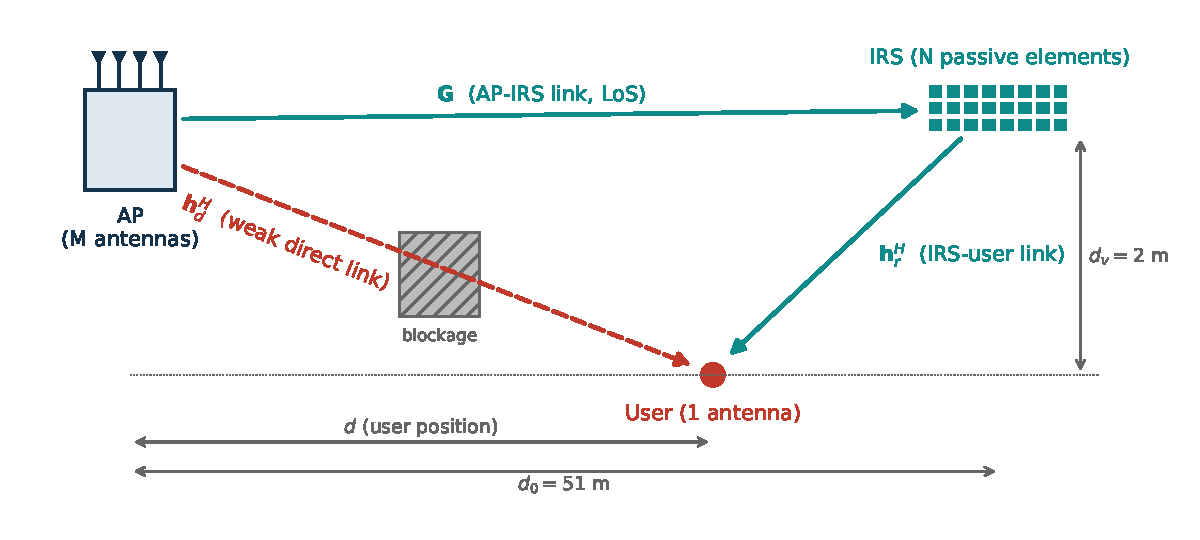
\includegraphics[width=0.85\linewidth]{system_model.pdf}
\caption{System model and the geometry used in our simulations. The user moves along a line parallel
to the AP--IRS line.}
\label{fig:model}
\end{figure}

The IRS is described by the diagonal matrix
$\Thm = \mathrm{diag}\!\left(e^{j\theta_1},\dots,e^{j\theta_N}\right)$, where $\theta_n\in[0,2\pi)$ is the
phase shift of element~$n$ and the reflection amplitude is one. The AP sends the symbol $s$, with
$\mathbb{E}|s|^2=1$, through the beamforming vector $\wv\in\mathbb{C}^{M\times1}$. The user receives
\begin{equation}
y = \left(\hrv^H \Thm\, \Gm + \hdv^H\right)\wv\, s + n ,
\label{eq:rx}
\end{equation}
where $n\sim\mathcal{CN}(0,\sigma^2)$ is the receiver noise. The first term inside the bracket is the
reflected path and the second is the direct path. The transmit power is $\|\wv\|^2$ and the received
signal-to-noise ratio (SNR) is $|(\hrv^H\Thm\Gm+\hdv^H)\wv|^2/\sigma^2$. Signals reflected by the IRS more
than once are neglected because of their high path loss, and the AP is assumed to know all channels.

\subsection{Problem formulation}

For an SNR target $\gamma$, the design problem is
\begin{align}
\text{(P1)}\qquad \min_{\wv,\,\bm{\theta}}\quad & \|\wv\|^2 \nonumber\\
\text{s.t.}\quad & \left|\left(\hrv^H\Thm\Gm+\hdv^H\right)\wv\right|^2 \ge \gamma\sigma^2, \label{eq:p1}\\
& 0\le\theta_n\le 2\pi,\quad n=1,\dots,N. \nonumber
\end{align}
The problem is non-convex because $\wv$ and $\Thm$ appear as a product in the constraint and because the
entries of $\Thm$ are restricted to the unit circle.

\subsection{Step 1: the transmit beamformer for fixed phases}

If the phases are fixed, the combined channel $\bm{h}^H = \hrv^H\Thm\Gm+\hdv^H$ is an ordinary
$1\times M$ channel. The beamformer that delivers a given SNR with the least power is maximum ratio
transmission (MRT),
\begin{equation}
\wv^\star = \sqrt{P}\,\frac{\left(\hrv^H\Thm\Gm+\hdv^H\right)^H}{\left\|\hrv^H\Thm\Gm+\hdv^H\right\|},
\qquad
P^\star = \frac{\gamma\sigma^2}{\left\|\hrv^H\Thm\Gm+\hdv^H\right\|^2}.
\label{eq:mrt}
\end{equation}
This is the same principle as maximum ratio combining: weight each antenna by the conjugate of its
channel so that all contributions add in phase. Substituting \eqref{eq:mrt} into (P1) removes $\wv$
and leaves a problem in the phases only,
\begin{equation}
\text{(P2)}\qquad \max_{\bm{\theta}}\ \left\|\hrv^H\Thm\Gm+\hdv^H\right\|^2
\quad\text{s.t.}\quad 0\le\theta_n\le2\pi .
\label{eq:p2}
\end{equation}
Minimising the transmit power is therefore the same as maximising the gain of the combined channel.

\subsection{Step 2a: semidefinite relaxation (SDR)}

Define $\vvec=[v_1,\dots,v_N]^H$ with $v_n=e^{j\theta_n}$ and $\Phm=\mathrm{diag}(\hrv^H)\,\Gm\in\mathbb{C}^{N\times M}$.
Then $\hrv^H\Thm\Gm=\vvec^H\Phm$, and
\begin{equation}
\left\|\vvec^H\Phm+\hdv^H\right\|^2 = \vvec^H\Phm\Phm^H\vvec + \vvec^H\Phm\hdv + \hdv^H\Phm^H\vvec + \|\hdv\|^2 .
\end{equation}
Introducing an auxiliary variable $t$ with $|t|=1$ and $\bar{\vvec}=[\vvec^T,\,t]^T$, this is the quadratic
form $\bar{\vvec}^H\Rm\,\bar{\vvec}+\|\hdv\|^2$ with
\begin{equation}
\Rm=\begin{bmatrix}\Phm\Phm^H & \Phm\hdv\\ \hdv^H\Phm^H & 0\end{bmatrix}.
\end{equation}
The constraint $|\bar v_n|=1$ is still non-convex. The idea of SDR is to \emph{lift} the problem to the
matrix $\Vm=\bar{\vvec}\bar{\vvec}^H$. Since $\bar{\vvec}^H\Rm\bar{\vvec}=\mathrm{tr}(\Rm\Vm)$, the objective is
linear in $\Vm$, and the unit-modulus constraints become $V_{nn}=1$. The matrix $\Vm$ must be positive
semidefinite and of rank one. Only the rank-one condition is non-convex. Dropping it gives
\begin{equation}
\text{(SDR)}\qquad \max_{\Vm}\ \mathrm{tr}(\Rm\Vm)
\quad\text{s.t.}\quad V_{nn}=1,\ n=1,\dots,N+1,\qquad \Vm\succeq 0,
\label{eq:sdr}
\end{equation}
which is a convex semidefinite programme (SDP) that standard solvers handle.

Because (SDR) optimises over a larger set than (P2), its optimal value is an upper bound on the
achievable channel gain. Through \eqref{eq:mrt} it gives a \textbf{lower bound on the transmit power}
that no scheme can beat. The solution $\Vm^\star$ generally has rank greater than one, so a feasible
phase vector is recovered by \emph{Gaussian randomisation}: with the eigen-decomposition
$\Vm^\star=\bm{U}\bm{\Sigma}\bm{U}^H$, draw $\bm{r}\sim\mathcal{CN}(\bm{0},\bm{I})$, form
$\bar{\vvec}=\bm{U}\bm{\Sigma}^{1/2}\bm{r}$, and set
$v_n=\exp\!\left(j\arg(\bar v_n/\bar v_{N+1})\right)$. This is repeated many times and the best
candidate is kept. The drawback of SDR is its cost: the SDP has $(N+1)^2$ unknowns, so the solve time
grows quickly with $N$.

\subsection{Step 2b: alternating optimisation}

To avoid the SDP, the paper proposes a low-complexity algorithm that alternates between the two sets of
variables.

\textbf{Phases for a fixed beamformer.} For a fixed $\wv$, the received amplitude is
$\left|\sum_{n} e^{j\theta_n}\,[\hrv^H]_n\,\bm{g}_n^H\wv + \hdv^H\wv\right|$, where $\bm{g}_n^H$ is the
$n$-th row of $\Gm$. By the triangle inequality this is largest when every term in the sum has the same
phase as the direct term, which gives the closed form
\begin{equation}
\theta_n^\star = \varphi_0 - \arg\!\left([\hrv^H]_n\,\bm{g}_n^H\wv\right),
\qquad \varphi_0=\arg\!\left(\hdv^H\wv\right).
\label{eq:phase}
\end{equation}

\textbf{Beamformer for fixed phases.} This is the MRT solution \eqref{eq:mrt}.

The algorithm starts from MRT towards the user, $\wv=\hdv/\|\hdv\|$, and repeats the two updates until
the relative decrease of the transmit power is below a threshold $\varepsilon$. Neither update can
increase the power and the power is bounded below, so the algorithm converges. Each iteration costs
only $\mathcal{O}(NM)$ operations.

Two simpler schemes are obtained by stopping after a single phase update with a fixed beam. In
\emph{AP--user MRT} the AP points at the user, $\wv\propto\hdv$. In \emph{AP--IRS MRT} the AP points at
the IRS. Both are used as benchmarks.

\subsection{The squared power scaling law}

To see how the gain grows with $N$, the paper considers a single-antenna AP, ignores the direct link,
and takes $\hrv\sim\mathcal{CN}(\bm{0},\varrho_h^2\bm{I})$ and $\bm{g}\sim\mathcal{CN}(\bm{0},\varrho_g^2\bm{I})$.
With the optimal phases \eqref{eq:phase} the received power is
$P_r = P\left(\sum_{n=1}^N |h_{r,n}|\,|g_n|\right)^2$. For large $N$ the sum is close to
$N\,\mathbb{E}|h_{r,n}|\,\mathbb{E}|g_n| = N\,\tfrac{\pi}{4}\varrho_h\varrho_g$, so
\begin{equation}
P_r \;\approx\; N^2\,\frac{\pi^2\varrho_h^2\varrho_g^2}{16}\,P .
\label{eq:n2}
\end{equation}
The received power grows with $N^2$. There are two reasons, each contributing one factor of $N$: the
surface \emph{collects} $N$ times more of the energy sent by the AP (aperture gain), and the $N$
reflected waves add \emph{coherently in amplitude} at the user (beamforming gain). For a fixed SNR
target the required transmit power therefore falls as $1/N^2$, that is, by $20\log_{10}2\approx6\udB$
each time $N$ is doubled. An active array of $N$ antennas with the same total transmit power gives a
gain of only $N$, or $3\udB$ per doubling.

\subsection{Extension to several users}

The paper also treats $K$ users served at the same time. Each user then has an SINR constraint that
includes the interference from the beams of the other users, and MRT is no longer optimal. The same
alternating idea is used. For fixed phases, the transmit beamformers are found from a standard
second-order cone programme (or with minimum mean-square-error beamforming). For fixed beamformers,
the phases are found from a feasibility problem that is again relaxed to an SDP. A lower-complexity
two-stage variant is also given. The main finding is that a well-configured IRS not only strengthens
the wanted signal near the surface but also helps to suppress interference between users. We studied
this part but restricted our simulations to the single-user case, as discussed in
Section~\ref{sec:limits}.

%=============================================================================
\section{Simulation and Reproduction of Results}
%=============================================================================

\subsection{Methodology}

We wrote the simulator from the equations above in Python (Appendix~\ref{app:code}). NumPy is used for
the channels and for the closed-form algorithms, CVXPY with the SCS solver for the SDP \eqref{eq:sdr},
and Matplotlib for the plots. The procedure is a Monte Carlo simulation:
\begin{enumerate}[leftmargin=1.6em,itemsep=2pt]
\item Place the user at horizontal distance $d$ from the AP (Fig.~\ref{fig:model}) and compute the three
link distances.
\item Draw one random realisation of $\Gm$, $\hrv$ and $\hdv$.
\item Compute the transmit power required by every scheme \emph{on the same channels}.
\item Repeat steps 2--3 many times, average the power in watts, and convert the average to dBm.
\end{enumerate}
The random seed is fixed, so the figures in this report can be regenerated exactly.

\textbf{Channel model.} The large-scale path loss of a link of length $d$ is
$L(d)=C_0\,(d/D_0)^{-\alpha}$ with reference distance $D_0=1$\,m. The AP--IRS link is assumed to be
line-of-sight (LoS), because the IRS is deployed where it has a clear view of the AP, so
$\Gm=\sqrt{L(d_0)}\,\bm{a}_N\bm{a}_M^H$, where $\bm{a}_N$ and $\bm{a}_M$ are the array responses of the
IRS and the AP with half-wavelength spacing. The IRS--user and AP--user links are Rayleigh fading,
that is, their entries are independent $\mathcal{CN}(0,L(\cdot))$. The direct AP--user link has the
largest path-loss exponent to represent blockage.

\textbf{Schemes compared.}
\begin{itemize}[leftmargin=1.4em,itemsep=1pt]
\item \emph{Lower bound}: the SDR optimum \eqref{eq:sdr} inserted in \eqref{eq:mrt}.
\item \emph{SDR + randomisation}: Section~2.4 with \nRand{} random candidates.
\item \emph{Alternating optimisation}: Section~2.5 with $\varepsilon=10^{-4}$.
\item \emph{AP--user MRT} and \emph{AP--IRS MRT}: fixed beam, phases from \eqref{eq:phase}.
\item \emph{Random phase shift}: random $\theta_n$, MRT on the resulting channel.
\item \emph{Without IRS}: $P=\gamma\sigma^2/\|\hdv\|^2$.
\end{itemize}

\subsection{Parameters}

Table~\ref{tab:params} lists the parameters. They follow the single-user setup of the paper as we
understood it. The points where our model is simpler than the paper's are discussed in
Section~\ref{sec:diff}.

\begin{table}[H]
\centering
\caption{Simulation parameters.}
\label{tab:params}
\begin{tabular}{ll}
\toprule
Parameter & Value \\
\midrule
Number of AP antennas, $M$ & \Msim \\
Number of IRS elements, $N$ & \Nsim{} (Experiments 1, 3); 10--160 (Experiments 2, 4) \\
AP--IRS distance, $d_0$ & 51 m \\
Vertical offset of the user line, $d_v$ & 2 m \\
Path loss at 1 m, $C_0$ & $-30$ dB \\
Path-loss exponent, AP--IRS & 2.0 \\
Path-loss exponent, IRS--user & 2.8 \\
Path-loss exponent, AP--user & 3.5 \\
Small-scale fading & AP--IRS: LoS; IRS--user and AP--user: Rayleigh \\
Noise power, $\sigma^2$ & $-80$ dBm \\
SNR target, $\gamma$ & 10 dB \\
Stopping threshold, $\varepsilon$ & $10^{-4}$ \\
Gaussian randomisations & \nRand \\
Channel realisations per point & \nReal{} (\nSdr{} for curves that need the SDP) \\
\bottomrule
\end{tabular}
\end{table}

\subsection{Experiment 1: transmit power versus user position}

Figure~\ref{fig:dist} shows the average transmit power as the user moves from the AP ($d=15$\,m) to
the IRS ($d=50$\,m), and Table~\ref{tab:dist} gives the numbers at selected positions.

\begin{figure}[H]
\centering
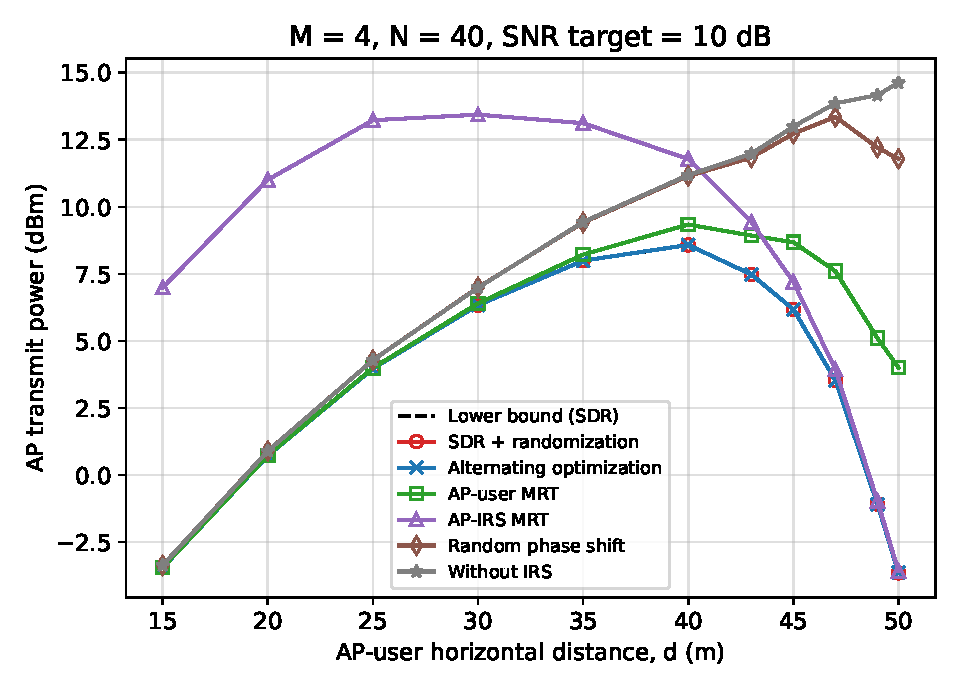
\includegraphics[width=0.74\linewidth]{fig1_power_vs_distance.pdf}
\caption{AP transmit power versus AP--user horizontal distance.}
\label{fig:dist}
\end{figure}

\begin{table}[H]
\centering
\caption{Average AP transmit power in dBm at selected user positions ($M=\Msim$, $N=\Nsim$).}
\label{tab:dist}
\tableDist
\end{table}

The curves can be read in three regions.

\emph{Near the AP.} The direct link is strong and the reflected link is weak, because the user is far
from the IRS. All schemes need almost the same power and the IRS brings little.

\emph{Between the AP and the IRS.} Without the IRS the power rises steadily with distance, as expected
from a path-loss exponent of 3.5. With the IRS the power also rises at first, reaches a maximum of
\peakP\udBm{} near $d=\peakD$\,m, where the user is far from both the AP and the IRS, and then falls.

\emph{Near the IRS.} The reflected link now dominates. At $d=50$\,m the jointly optimised system needs
\aoFifty\udBm{} against \noIrsFifty\udBm{} without the IRS, a saving of \saveFifty\udB. The IRS thus
creates a ``signal hotspot'' around itself, and a user at the cell edge can be served with less power
than a user in the middle of the cell.

The comparison between schemes is also instructive.
\begin{itemize}[leftmargin=1.4em,itemsep=2pt]
\item The alternating optimisation and SDR with randomisation both lie on the lower bound (the largest
gap is \gapLB\udB). The cheap closed-form algorithm is therefore practically optimal in this setup.
\item AP--user MRT is close to optimal near the AP but loses \gapUserMRT\udB{} at $d=50$\,m, because it
sends its energy towards the user and too little of it reaches the IRS.
\item AP--IRS MRT shows the opposite behaviour. It is close to optimal near the IRS but loses
\gapIrsMRT\udB{} at $d=15$\,m, because it ignores the strong direct link.
\item With random phases the reflected waves add incoherently, and the result is \gapRand\udB{} worse
than the joint design at $d=50$\,m. The benefit of an IRS comes from the phase design and not from
the mere presence of a reflector.
\end{itemize}
No single fixed beam is good everywhere. The joint design balances the energy sent towards the user
and towards the IRS according to the user position.

\subsection{Experiment 2: transmit power versus number of IRS elements}

Figure~\ref{fig:N} tests the scaling law \eqref{eq:n2} for three user positions.

\begin{figure}[H]
\centering
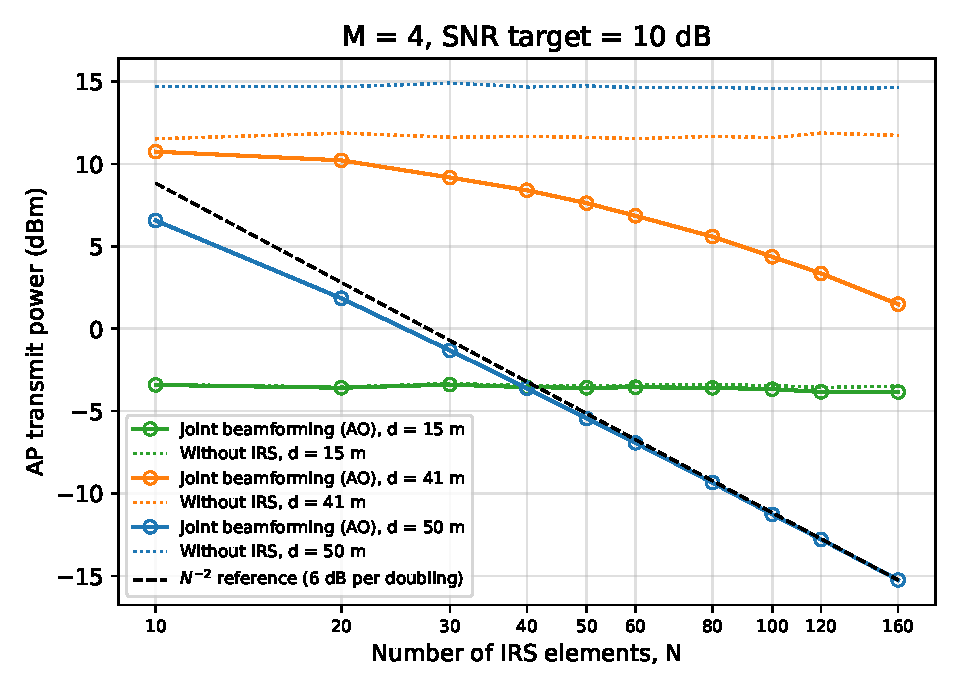
\includegraphics[width=0.74\linewidth]{fig2_power_vs_N.pdf}
\caption{AP transmit power versus the number of IRS elements. The dashed line has the slope of the
$1/N^2$ law.}
\label{fig:N}
\end{figure}

For the user next to the IRS ($d=50$\,m) the curve is parallel to the dashed $N^{-2}$ reference.
Increasing $N$ from 40 to 80 reduces the power by \dropA\udB, and from 80 to 160 by \dropB\udB, against
the theoretical 6.0\udB{} per doubling. This confirms the squared power gain. It is worth noting that
the law holds here even though the direct link is present and $M>1$, which are not covered by the
simplified derivation: near the IRS the reflected link is simply much stronger than the direct one.

For the user near the AP ($d=15$\,m) the power changes by only \dropFifteen\udB{} over the whole range
of $N$, because the direct link dominates and the IRS is far away. The user at $d=43$\,m lies between
the two cases. Its curve is flat for small $N$ and steepens as $N$ grows and the reflected link starts
to dominate. An IRS is therefore most useful for users that are close to it and poorly served by the
AP, and its size must be large enough for the reflected link to overtake the direct one.

\subsection{Experiment 3: convergence of the alternating optimisation}

Figure~\ref{fig:conv} shows the transmit power after each iteration of the alternating optimisation
for a user at $d=45$\,m, together with the SDR lower bound. Iteration~0 is the starting point,
AP--user MRT. To see how the channel affects convergence we varied the Rician factor $K$ of the
AP--IRS link from pure LoS ($K=\infty$) to Rayleigh ($K=0$).

\begin{figure}[H]
\centering
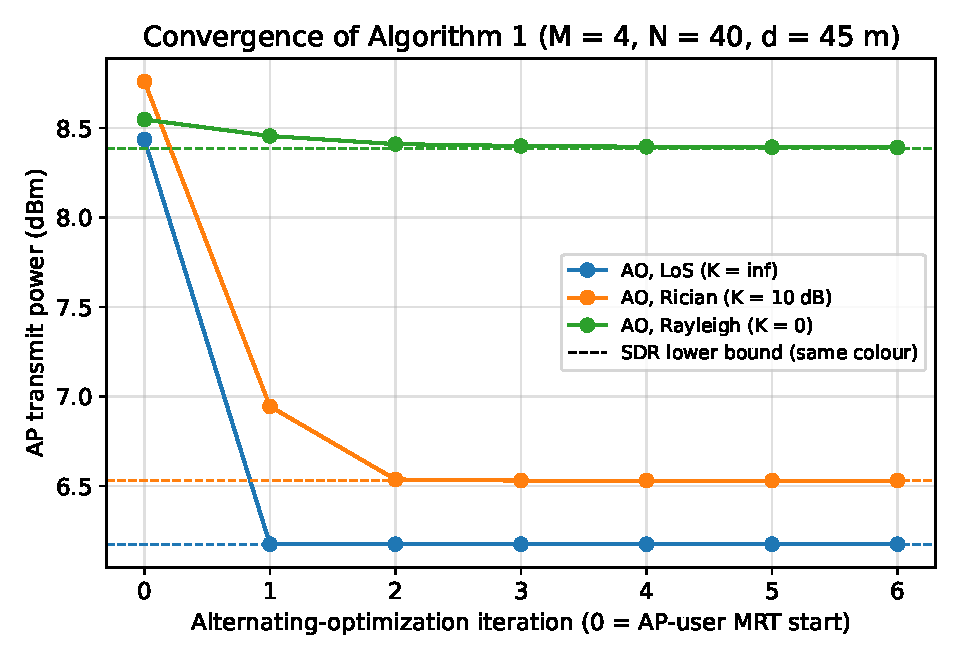
\includegraphics[width=0.72\linewidth]{fig3_convergence.pdf}
\caption{Convergence of the alternating optimisation for different AP--IRS channels. Dashed lines:
SDR lower bounds.}
\label{fig:conv}
\end{figure}

The power decreases monotonically in every case, as the theory requires. With a LoS AP--IRS link the
algorithm reaches the lower bound after a \emph{single} iteration. This surprised us at first, and we
found the reason: when $\Gm=\sqrt{L}\,\bm{a}_N\bm{a}_M^H$ has rank one, the reflected channel is
$\hrv^H\Thm\Gm=z\,\bm{a}_M^H$ with the single complex number
$z=\sqrt{L}\sum_n e^{j\theta_n}[\hrv^H]_n[\bm{a}_N]_n$, and
\begin{equation}
\left\|z\,\bm{a}_M^H+\hdv^H\right\|^2 = M|z|^2 + 2\,\mathrm{Re}\!\left(z\,\bm{a}_M^H\hdv\right) + \|\hdv\|^2 .
\end{equation}
This is maximised by making $|z|$ as large as possible, which means aligning all $N$ terms, and by
choosing the common phase of $z$ to cancel that of $\bm{a}_M^H\hdv$. The phase update \eqref{eq:phase}
with the initial beam $\wv\propto\hdv$ produces exactly this solution. With a rank-one $\Gm$ the problem
therefore has a closed-form optimum, which also explains why the three best curves coincide in
Fig.~\ref{fig:dist}.

When the AP--IRS channel has a scattered component, more iterations are needed, but convergence is
still fast: for the Rayleigh case the power after six iterations is within \gapRay\udB{} of the lower
bound. The gain of the IRS is also much smaller in that case, because a full-rank random $\Gm$ does not
let the $N$ reflections be aligned for all AP antennas at once. This supports the usual advice to
place the IRS in line of sight of the AP.

\subsection{Experiment 4 (our extension): finite-resolution phase shifters}

The paper assumes that each phase can take any value. Practical elements offer only $2^b$ levels. As
an addition of our own we quantised the optimised phases to $b$ bits and recomputed the power
(Fig.~\ref{fig:disc}).

\begin{figure}[H]
\centering
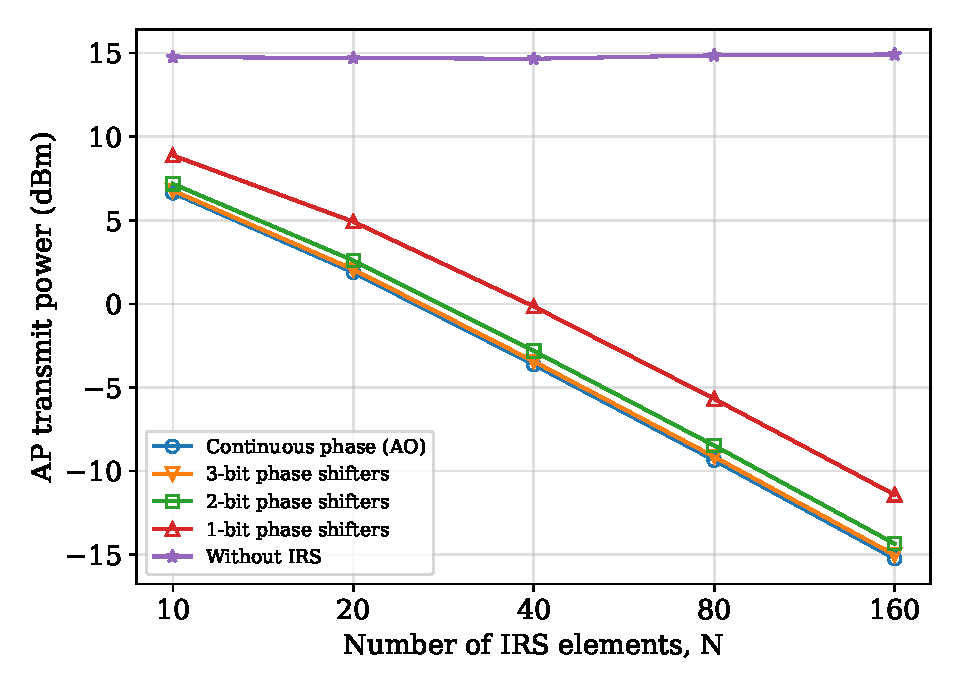
\includegraphics[width=0.72\linewidth]{fig4_discrete_phase.pdf}
\caption{Effect of phase quantisation for a user at $d=50$\,m.}
\label{fig:disc}
\end{figure}

At $N=160$ the loss with respect to continuous phases is \lossOne\udB{} for 1-bit elements,
\lossTwo\udB{} for 2 bits and \lossThree\udB{} for 3 bits. All curves keep the same slope, so the squared
power gain survives quantisation: a coarse phase error reduces the coherent sum by a constant factor
but does not change how it grows with $N$. Two bits per element already recover almost all of the
gain, which is encouraging for low-cost hardware.

\subsection{Comparison with the results in the paper}
\label{sec:diff}

Our simulations reproduce the qualitative results of the single-user part of the paper:
\begin{itemize}[leftmargin=1.4em,itemsep=2pt]
\item the transmit power first rises and then falls as the user moves from the AP towards the IRS,
while it only rises without the IRS;
\item the joint design achieves the SDR lower bound, and the alternating optimisation performs as well
as SDR with randomisation at a small fraction of the cost;
\item AP--user MRT is near-optimal close to the AP and AP--IRS MRT close to the IRS, and each is
clearly sub-optimal in the other region;
\item the transmit power near the IRS falls by about 6\udB{} when $N$ is doubled.
\end{itemize}

The absolute power levels need not coincide with those in the paper, for the following reasons.
\begin{enumerate}[leftmargin=1.6em,itemsep=2pt]
\item \textbf{Antenna and element gains.} We use isotropic (0\,dBi) antennas and elements. Any gain
assumed for the AP antennas or the reflecting elements shifts the curves vertically without changing
their shape.
\item \textbf{Array geometry.} We model both the AP and the IRS as uniform linear arrays to generate
the LoS response. With a rank-one LoS channel the optimal power depends only on the magnitudes of the
entries, so this does not affect the averages, but it is a difference in the model.
\item \textbf{Parameter values.} The values in Table~\ref{tab:params} follow our reading of the paper.
A different number of AP antennas, number of elements or Rician factor in a particular figure of the
paper would change the corresponding curve.
\item \textbf{Monte Carlo accuracy.} The SDP-based curves use \nSdr{} channel realisations, which
leaves a statistical uncertainty of a few tenths of a dB, mainly in the ``without IRS'' curve, where a
single deep fade of the direct link has a large effect on the average.
\item \textbf{Solver.} We solve the SDP with the first-order solver SCS at a tolerance of $10^{-5}$,
whereas the paper uses CVX. The resulting difference in the lower bound is far below the plotting
resolution.
\item \textbf{Scope.} We did not simulate the multiuser results of the paper.
\end{enumerate}

%=============================================================================
\section{Conclusion}
%=============================================================================

\subsection{Key outcomes and findings}

The paper shows that a passive reflecting surface, configured jointly with the transmit beamformer,
can reduce the transmit power needed to serve a user by a large amount. For a single user the optimal
beamformer is MRT on the combined channel, so the problem reduces to choosing the IRS phases. The
paper gives a semidefinite relaxation that provides a performance bound and a near-optimal solution,
and a closed-form alternating algorithm with very low complexity. It also proves that the received
power grows with the square of the number of elements.

Our own simulations confirm these findings. With $M=\Msim$ and $N=\Nsim$, a user next to the IRS needs
\saveFifty\udB{} less transmit power than without the IRS. The alternating optimisation is within
\gapLB\udB{} of the lower bound. Doubling $N$ saves \dropA--\dropB\udB{} near the IRS, in agreement with
the 6\udB{} predicted by the $N^2$ law. In addition we found that the algorithm is exactly optimal in
one step when the AP--IRS channel is LoS, and that 2-bit phase shifters lose only \lossTwo\udB.

\subsection{Difficulties encountered and how we addressed them}

\textbf{Understanding the optimisation tools.} Semidefinite relaxation, lifting and Gaussian
randomisation are outside our course. We first solved the cases $N=1$ and $N=2$ by hand, where the
optimal phases are obvious, and used them to understand the general matrix formulation. A tutorial
article on SDR~\cite{luo} was also helpful.

\textbf{Computation time.} Our first implementation used an interior-point solver and needed about
10 seconds per channel realisation for $N=40$, while a smooth curve needs thousands of realisations.
We changed to a first-order solver, which was more than ten times faster, ran the different user
positions in parallel on separate processor cores, and used the SDP only in the experiments where the
bound is needed. The closed-form schemes take a fraction of a millisecond per realisation.

\textbf{Verifying the code.} A sign error in a phase or a missing conjugate still gives a
plausible-looking curve. We therefore relied on three independent checks: the alternating optimisation
must never fall below the SDR lower bound and should be close to it; the ``without IRS'' curve must
agree with the value expected from the path-loss model; and the slope against $N$ must be 6\udB{} per
doubling. The Hermitian-transpose conventions ($\hdv$ versus $\hdv^H$) caused several early mistakes
that these checks exposed.

\textbf{An unexpected result.} The three best schemes gave identical results to several decimal
places, which looked like a programming error. Working through the algebra for a rank-one $\Gm$
(Section~3.5) showed that this is the correct behaviour.

\subsection{Limitations and future directions}
\label{sec:limits}

\begin{itemize}[leftmargin=1.4em,itemsep=2pt]
\item \textbf{Channel knowledge.} The paper, and our simulation, assume that all channels are known
perfectly. A passive IRS cannot transmit or process pilots, so only the cascaded channel can be
estimated, and the training overhead grows with $N$. Channel estimation is the main practical obstacle.
\item \textbf{Ideal hardware.} Continuous, lossless phase shifts that are independent of the reflection
amplitude are assumed. Real elements have a few discrete levels, some loss, and coupled amplitude and
phase. Our fourth experiment addresses only the first of these.
\item \textbf{Channel model.} The model is narrowband, far-field and single-cell. In a wideband OFDM
system one set of phases must serve all subcarriers, and a very large surface may operate in the near
field.
\item \textbf{Range of the scaling law.} The $N^2$ gain appears only once the reflected link dominates
the direct link, and it cannot continue without limit, since the surface cannot deliver more power
than it intercepts.
\item \textbf{Scope of our reproduction.} We reproduced the single-user results only. Simulating the
multiuser algorithms of the paper is the natural next step.
\end{itemize}

Later work has followed several of these directions: beamforming with discrete phase
shifts~\cite{wu_discrete}, channel estimation methods with reduced overhead, multi-IRS and wideband
designs, active and simultaneously transmitting-and-reflecting surfaces, and learning-based phase
control. The joint design studied here remains the starting point for these.

%=============================================================================
\begin{thebibliography}{9}
\bibitem{wu} Q.~Wu and R.~Zhang, ``Intelligent reflecting surface enhanced wireless network via joint
active and passive beamforming,'' \emph{IEEE Trans. Wireless Commun.}, vol.~18, no.~11,
pp.~5394--5409, Nov. 2019.
\bibitem{wu_mag} Q.~Wu and R.~Zhang, ``Towards smart and reconfigurable environment: Intelligent
reflecting surface aided wireless network,'' \emph{IEEE Commun. Mag.}, vol.~58, no.~1, pp.~106--112,
Jan. 2020.
\bibitem{wu_discrete} Q.~Wu and R.~Zhang, ``Beamforming optimization for wireless network aided by
intelligent reflecting surface with discrete phase shifts,'' \emph{IEEE Trans. Commun.}, vol.~68,
no.~3, pp.~1838--1851, Mar. 2020.
\bibitem{luo} Z.-Q.~Luo, W.-K.~Ma, A.~M.-C.~So, Y.~Ye, and S.~Zhang, ``Semidefinite relaxation of
quadratic optimization problems,'' \emph{IEEE Signal Process. Mag.}, vol.~27, no.~3, pp.~20--34,
May 2010.
\bibitem{goldsmith} A.~Goldsmith, \emph{Wireless Communications}. Cambridge, U.K.: Cambridge
University Press, 2005.
\bibitem{tse} D.~Tse and P.~Viswanath, \emph{Fundamentals of Wireless Communication}. Cambridge, U.K.:
Cambridge University Press, 2005.
\end{thebibliography}

%=============================================================================
\appendix
\section{Simulation code}
\label{app:code}
The complete simulator is listed below. It requires Python~3 with NumPy, Matplotlib and CVXPY, and is
run with \texttt{python ris\_sim.py}.

\lstinputlisting{ris_sim.py}

\end{document}
